\documentclass[11pt, oneside]{article}   	% use "amsart" instead of "article" for AMSLaTeX format
\usepackage{geometry}                		% See geometry.pdf to learn the layout options. There are lots.
\geometry{letterpaper}                   		% ... or a4paper or a5paper or ... 
%\geometry{landscape}                		% Activate for rotated page geometry
%\usepackage[parfill]{parskip}    		% Activate to begin paragraphs with an empty line rather than an indent
\usepackage{graphicx}				% Use pdf, png, jpg, or eps§ with pdflatex; use eps in DVI mode
								% TeX will automatically convert eps --> pdf in pdflatex		
\usepackage{amssymb}

\usepackage{ dsfont }

%SetFonts

%SetFonts


%\title{Brief Article}
%\author{}
%\date{}							% Activate to display a given date or no date

\begin{document}
%\maketitle
%\section{}
\subsection*{Note:} $h_o(x) = g(\theta^Tx) = g(x_1\theta_1 + ... + x_j\theta_j + ... x_n\theta_n)$ , \hspace{1cm} ($z = {x_1\theta_1 + ... + x_j\theta_j + ... x_n\theta_n}$) \

$\frac{\partial}{\partial\theta_j} h_o(x) = g'(z) \frac{\partial z}{\partial\theta_j} $ , \hspace{5cm} $x_j = \frac{\partial z}{\partial\theta_j} $ \

$g(z) = \frac{1}{1 + e^-z}$\

$g'(z) = \frac{e^{-z}}{1 + e^{-z}} = \frac{1}{1 + e^{-z}} \frac{e^{-z}}{1 + e^{-z}} = g(z)(1-g(z))$\

($\therefore 1 - g(z) = 1 - \frac{1}{1 + e^{-z}} = \frac{e^{-z}}{1 + e^{-z}}$)\\

\subsection*{Stochastic Gradient Descent:}

$\theta_j := \theta_j + \alpha \frac{\partial}{\partial \theta_j} l(0) = \theta_j + \alpha (y^{(i)} - h(x^{(i)})x_j^{(i)})$ \\

There is another method which runs faster than this stochastic gradient descent method. It it called Newton's method.

\subsection*{Newton's Method:} 

Say $f : \mathds{R} \to \mathds{R}$ \

 $f(x_{n+1}) = f(x_{n+1}) = f(x_n) + f'(x_n)t + \frac{1}{2} f''(x_n)t^2$

$\frac{df}{dt}(x_{n+t}) = f'(x_n) + \frac{1}{2} f''(x_n)2t = 0$

$\frac{df}{dt}(x_{n+t}) = f'(x_n) + f''(x_n)t = 0$ \\

$t = \frac{-f'(x_k)}{f'(x_k)}$ \hspace{1mm} $x_{k+1} = x_k - \frac{f'(x_k)}{f'(x_k)}$


\begin{figure}[htbp] %  figure placement: here, top, bottom, or page
   \centering
   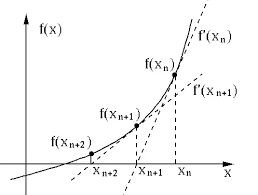
\includegraphics[width=3.5in]{nm.png} 
   \caption{Newton's Method}
   %\label{Newton's Method}
\end{figure}







\end{document}  